\section{Display 2.0}
This explains the display
\begin{figure}
	\begin{center}
		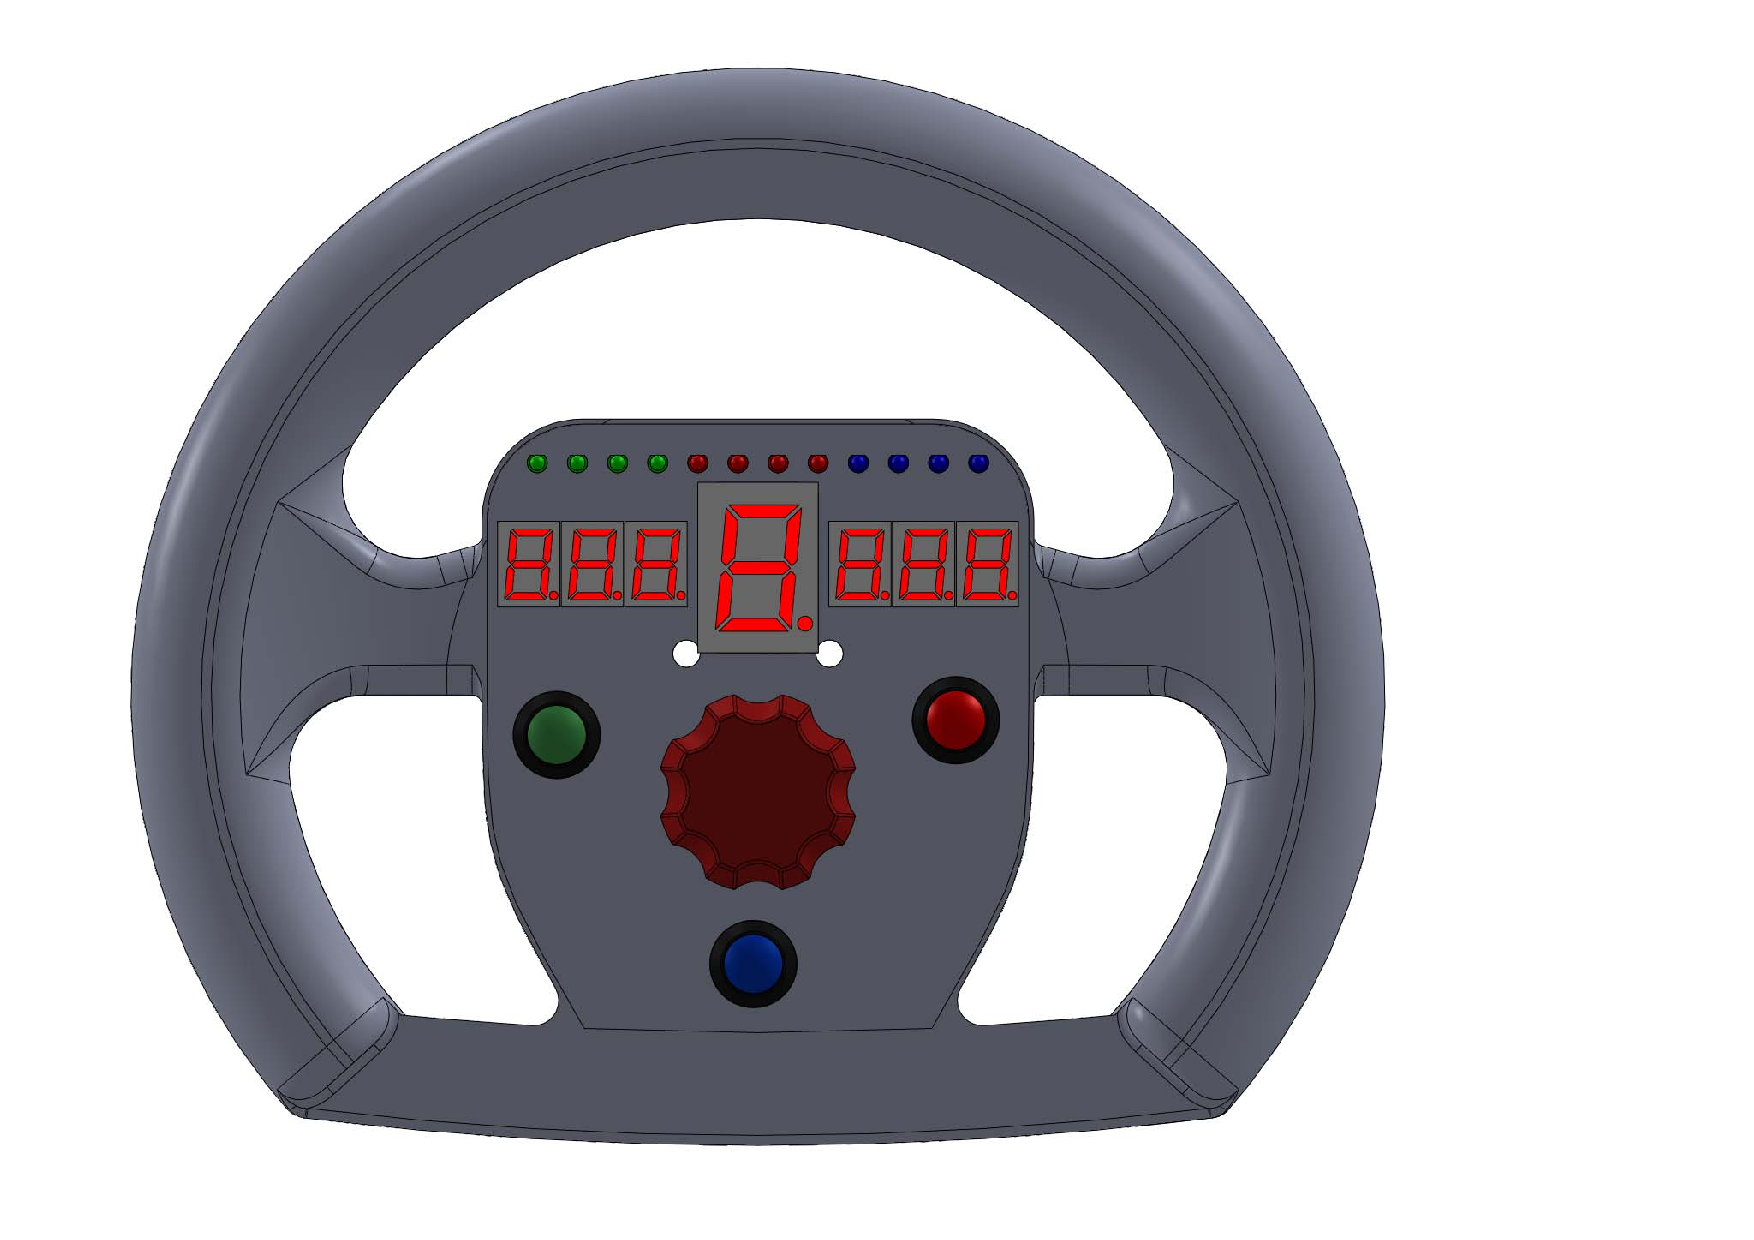
\includegraphics[scale=0.3]{G6SteeringWheelV3.pdf}
		\caption{Concept drawing of steering wheel with display, not final edition}
	\end{center}
\end{figure}
\section{graphical overview}
\subsection*{RPM Measurement}
At the top of the steering wheel there is located 20 LED's in assorted colors, in the order of Green, Red, Blue. These are designed to be individually phase line controlled in the order of lighting op from left to right.

\subsection*{Shift-light}
Large brigt blue LED positioned underneath the RPM lights, meant for indicating optimal gear shift upwards and downwards. This ligths need to take into account the current RPM of the engine, and the RPM of the wheels, and human reaction time.

\subsection*{Seven segment multi display}
seven seven-segment displays placed underneath shift light, divided into 3 groups.\newline
Left group is the first 3 segment from the left, meant to show user selectable info from CAN. Segment color is red\newline
Middle segment i the fourth from the left, and is meant to show the estimate of the current gear position. Segment color is green\newline
Right group is the last 3 segments from the left, meant to show user selectable info from CAN. Segment color is red.\newline
Left group and right group wil have same size segments, and middle group will have slightly larger segment for easier reading.

\subsection*{RGB status indicator light}
The lights will light up in three different modes:

\begin{enumerate}
	\item[•]Green = Good
	\item[•]Red = Bad
	\item[•]Blinking blue = Critically bad
\end{enumerate}
Description of the indication of the LED's:
Light number one is left most, and number eight is right most
\begin{center}
  \begin{tabular}{| c | c | c | c | c |}
    \hline
    LED & Indication & Good value & Bad value & Critical value \\ \hline
    1 & Battery Voltage & <12 & >12 & >10 \\ \hline
    2 & Water Temperature & >80 & >100 & <100  \\ \hline
    3 & Oil Temperature & xx & xx & xx \\ \hline
    4 & Oil Pressure & High & xx & Low / No readings \\ \hline
    5 & Air Temperature & xx & xx & xx \\ \hline
    6 & Air Pressure & xx & xx & xx \\ \hline
    7 & Fuel & High & Low & xx \\ \hline
    8 & Launch control & On & OFF & xx \\ \hline
  \end{tabular}
\end{center}

\subsection*{Buttons}
The buttons on the steering wheel consists of the following:
\begin{center}
  \begin{tabular}{| c | c | c | c |}
    \hline
    Function & Placement & Type & Reachable while driving  \\ \hline
    Launch control & Upper left & momentary push(LED) & Yes\\ \hline
    Tranction control (quick disable) & Upper right & Momentary push(LED) & Yes\\ \hline
    Seven segment side select & Upper middle & 3 stage spring loaded & Yes\\ \hline
    Seven segment info select & Upper middle & 12/16 stage rotary switch & Yes\\ \hline
    Neatral gear enable & Lower middle & Momentary push & Yes(hardly)\\ \hline
    Traction control (mode select) & Buttom back & 2 stage rocker & No\\ \hline
    RPM (mode select [Full or 3-segmented]) & Buttom back & 2 stage rocker & No\\ \hline
    
  \end{tabular}
\end{center}
Written by Henrik Jensen \& Peter Reichwald. 